\documentclass[
pdftex,                %PDFtext verwenden
a4paper,                 %A4Papier
11pt,                     %Schriftgröße 12
parskip=half,         %Halbe Zeile Abstand zwischen den Paragraphen
headsepline,        %Linie nach Kopfzeile
]
{scrartcl}

\usepackage{graphicx}	% Paket um Grafiken einbetten zu können
\usepackage{color}	% Package für Farben im PDF
\usepackage{amsmath}
\usepackage{makeidx}	% Paket für die Indexerstellung
\usepackage[a4paper,left=2.0cm,right=2.0cm]{geometry}	%Paket zum Einstellen der Seitenränder
\usepackage[T1]{fontenc}	% Verwenden von T1 Fonts
\usepackage[urlcolor=blue]{hyperref}
\usepackage{caption}	% Caption verändern
\usepackage{verbatim}
\usepackage{booktabs}

%\setcapwidth[r]{\linewidth}

\begin{document}
	
	\newcommand{\group}{Group C - The Plebs}
	
	\newcommand{\header}{Python Chess AI}

	\pagestyle{myheadings}
	\markright{\group \hfill \header}
	
	\thispagestyle{empty}
	\begin{titlepage}

    Course: Project AI - Symbolic artificial intelligence \\
    Professor: Dr.-Ing. Stefan Fricke \\
    Semester: SOSE23 \\
    Date: 2023/07/26 \\

    Group Members: Who the fuck cares? \\
    Repository: https://github.com/PraxTube/chess-ai/ \\
		
		\vspace{8mm}
		
		\begin{center}
			
			{\Large \normalfont \bfseries Project Report} \\
			
			\vspace{5mm}
			
			{\Huge \normalfont \bfseries \header} \\
			\vspace{7mm}
			
			{\Large \normalfont \bfseries \group} \\
			\vspace{5mm}
			
		\end{center}
		\vspace{2cm}
		
		\begin{abstract}
			
			This is a dummy abstract.

Hello there.

			
		\end{abstract}
		
	\end{titlepage}
	
	\pagenumbering{Roman}
	
	\tableofcontents
	
	\pagebreak
	
	\pagenumbering{arabic}\setcounter{page}{1}

  \section{Introduction}

  Creating a chess AI from scratch is quite a challenging undertaking.
Not only will you need to write a whole chess backend, you will also
need to implement the AI features. One of the major issues here
is to write a chess backend without any bugs and to test your
AI properly to make sure the features you add actually make it
play better.

Our group chose to use Python for the whole project given
that that is what we were most familiar with.
The obvious trade-off here is of course that it's easy
to prototype but painfully slow and very error prone.
I personally would have liked to try to use Rust,
though in hindsight we would have probably abandoned
the project if we had used Rust simply because
the chess engine alone was so much work.
On the other side I have acquired some Rust experience
now and if I were to write the chess engine
(or something of a similar level) I would probably
go with Rust.

Regardless of our programming language, for version control
we obviously used git and to share our code base we used github.
The overall workflow here was pretty smooth.

This was pretty much the first \textit{real} AI project we
took on. Our goal was to at least get a basic AI done,
that was what we wanted to to reach at least.
Our final AI is actually fairly advanced for what we seeked
to accomplish. It's obviously not the strongest (
given that we are using python that isn't too surprising).
However we are very pleased with the end result and with what
we created and learned during this project.

In the following chapters we will go into more detail
into what, why and how we created our AI.
We will also reflect on all these things.


  \pagebreak

  \section{Development}

  Before we are going into the details of the
development process let's first look at
the high level overview of what we created
(note that you can click on the Mst name to see
whole documentation of it).

\begin{description}
  \item[\href{https://github.com/PraxTube/chess-ai/tree/master/docs/milestones/1-dummy-AI}{Mst1 - Dummy AI:}] \hfill
    \begin{itemize}
      \item Chess Backend
      \item Dummy AI (minimax)
      \item Basic Evaluation (Material only)
    \end{itemize}
  \item[\href{https://github.com/PraxTube/chess-ai/tree/master/docs/milestones/2-basic-AI}{Mst2 - Basic AI:}] \hfill
    \begin{itemize}
      \item Improve Backend
      \item Alpha-Beta Tree Search
      \item Improved Evaluation (PeSTO)
      \item Better time management
    \end{itemize}
  \item[\href{https://github.com/PraxTube/chess-ai/tree/master/docs/milestones/3-advanced-AI}{Mst3 - Advanced AI:}] \hfill
    \begin{itemize}
      \item Restructured Chess Backend
      \item Speed up Evaluation (through numpy)
      \item Improve move ordering
      \item Include King of the Hill in evaluation
      \item Restructure internal debug info
    \end{itemize}
  \item[\href{https://github.com/PraxTube/chess-ai/blob/documentation-milestone-four/docs/milestones/4-optimized-AI/README.md}{Mst4 Optimized AI:}] \hfill
    \begin{itemize}
      \item Improve evaluation
      \item Use Monte Carlo Tree Search
      \item Implement PVS/negamax
      \item Add Nullsearch
    \end{itemize}
\end{description}

\pagebreak

\subsection{Mst1 Dummy AI}




  \pagebreak

  \section{Results}

  In this section we will focus on the benchmarks
and the more tangible results of the project.
The tests were run on a PC with the following specs

\begin{itemize}
  \item CPU: Intel i5-4590, Threads: 4, Cores: 4, 3.7GHz
  \item RAM: 24GB DDR3
  \item OS: Zorin 16.2 (Ubuntu based)
\end{itemize}

To start, lets take a look at \autoref{fig:pillar-plot}.

\begin{figure}[hbtp]
	\centering
	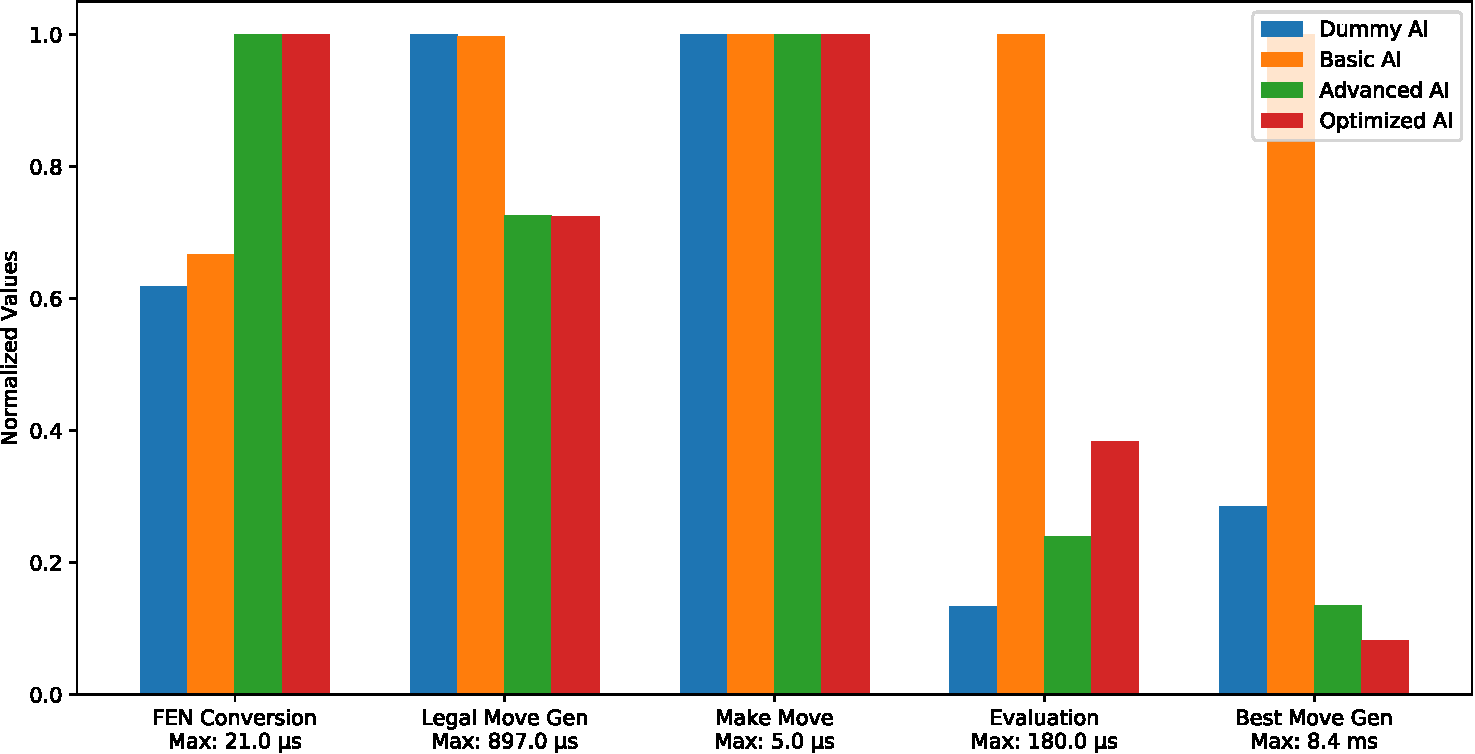
\includegraphics[width=.9\linewidth, page=1]{reference/pics/plot.pdf}
	\caption{Benchmarks of the different categories across the AI versions.}
	\label{fig:pillar-plot}
\end{figure}

We can see five categories, of which the first three
are determined by the chess backend and the later two
by the AI.
Important to note in the backend benchmarks is the legal move
generation. This is the main bottleneck of the backend
and a increasing the performance there has quite
the effect on the overall performance of the AI.
The decrease in time stems from the refactor of using
lists of integers and reducing boilerplate\footnote{
The Fen conversion is only used for debugging
purposes, the fact that it increased is not noticeable
in an optimized AI that doesn't debug anything.}.
The most important category however is the last one,
the \textit{Best Move Generation}. As the name suggests,
this indicates how fast the AI calculated the best move,
here at a depth of one.
The optimized AI has the best overall time,
even though it's slower in the evaluation compared to
the previous version. This illustrates very nicely
that the end result of an AI, it's strength and speed,
is determined by multiple factors. In this case
the amount of nodes searched was drastically decreased
by the AI features implemented which led to this
overall improvement.

\pagebreak

This leads us to \autoref{fig:depth-plot}, which shows
the time and number of nodes searched in respect to the
depths. Here we can see numbers of nodes searched (bottom plot) is significantly
lower for the optimized AI compared to the advanced AI\footnote{
The reason the dummy and basic AI seem to have less nodes searched
is because there was a bug in the early implementations of the AI.
This bug had to do with the move ordering and was fixed in milestone three.
For that reason the dummy and basic AI's benchmarks in regard to depth
should be taken with a grain of salt.
}. We can also see that the overall time is smaller for the optimized AI,
regardless of depth.

This is actually not necessarily the case,
for instance if we would have made poor decisions for the MCTS
with regard to exploration/exploitation and this could have actually been
slower for higher depths. This is where regular benchmarks, or atomic
benchmarks are very useful, you change one little nod and see how the
system responds. Research also helped to fine tune.

\begin{figure}[hbtp]
	\centering
	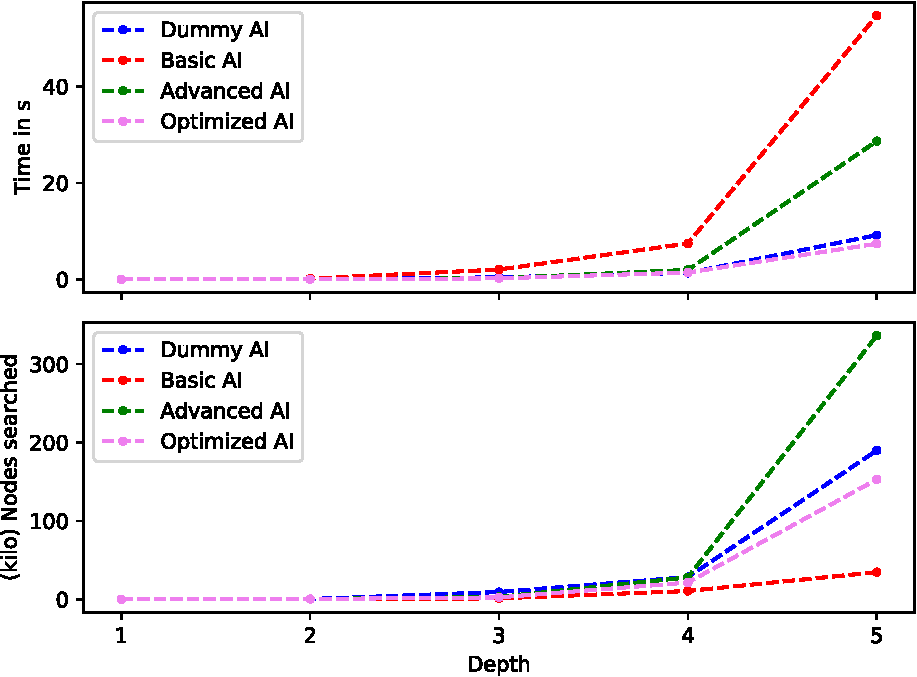
\includegraphics[width=.8\linewidth, page=1]{reference/pics/plot-depths.pdf}
	\captionsetup{justification=centering}
	\caption{Benchmarks of different AI versions in respect to search depth.\\Note that the number of nodes searched is in thousands (kilo).}
	\label{fig:depth-plot}
\end{figure}

\pagebreak


  \section{Issues faced}

  This section presents a compilation of challenges we encountered throughout the project. While they are not arranged in a specific order, they implicitly follow the sequence of milestones from one to four.

\begin{itemize}
\item Balancing the trade-off between the ease of prototyping in Python and its slower execution speed.
\item Working with Object-Oriented Programming (OOP) can be challenging, particularly when the software design lacks clarity.
\item The process of writing and debugging the chess engine was challenging. A more structured approach would have been preferable to trial and error.
\item Early unit testing proved to be less beneficial than anticipated.
\item The initial phase was the most difficult, as we were uncertain about where to begin.
\item The indiscriminate use of numpy does not automatically enhance code performance and can, in fact, slow it down.
\item Dealing with extensive functions with large logical statements.
\item Implementing advanced AI algorithms, such as Principal Variation Search (PVS) and Monte Carlo Tree Search (MCTS), in a way that effectively improved the AI's performance.
\item Dealing with the complexities of implementing a transposition table, including handling hash collisions.
\item Ensuring the accuracy and efficiency of the AI's evaluation process, particularly when introducing new features.
\item Managing the project's scope and complexity, especially when adding new features or making significant changes to the AI or backend.
\item Overcoming the limitations of the initial AI framework and restructuring it to accommodate new features.
\item Making multiple changes simultaneously, as opposed to implementing atomic changes.
\item Committing to tasks that ultimately did not yield significant benefits.
\item Coordinating team efforts, primarily due to the fact that the engine could effectively be worked on by only one person at a time.
\item Navigating and resolving GitHub merge conflicts among team members, which required a clear understanding of the code changes made by each individual and effective communication to ensure that important updates were not inadvertently discarded.
\end{itemize}

Despite these challenges, most provided valuable learning opportunities. The lessons we gleaned from this project will be discussed in the subsequent chapter.


  \section{Lessons learned}

  The process of writing a chess AI is not an easy one.
There are many things that can and will go wrong.
That's why this was a great way to learn,
because the first step to mastery is failure.
The following list is a collection of lessons we learned during
this project, they are in no particular order.

\begin{itemize}
  \item{
Benchmarks are extremely useful,
not only to see improvements over different versions of your code,
but also to compare incremental changes to the code.
We realized this when we tried to refactor the evaluation function to use numpy.
When we had many small np.ndarray it was actually slower then the pure python list implementation.
This is because we always have overhead when calling numpy,
so reducing the amount of times we call numpy draws out the full potential of numpy,
i.e. use as big as arrays as possible.
}
  \item{
We also observed that background tasks can significantly influence the result of benchmarks.
One should try to run them in the same-ish environment as possible
(or use a server for that if possible).
}
  \item{
Writing debugging tools as early as possible really pays off (same with logging tools).
}
  \item{
Failing fast in the early stages of the project (using python-chess to code up a simple AI)
created a good base knowledge about what needs to be done.
}
  \item{
Writing good git commits is extremely useful for both documentation and overall work flow.
Atomic commits are almost necessary when restructuring complex software like the chess backend.
}
  \item{
Unit tests really useful when restructuring complex software as well.
}
  \item{
It's important to know if something will be worthwhile
before commiting to it if it will take a long time to complete.
We learned this with the attempt at implementing transposition tables.
If we would have known that the potential performance increase was about
\~10\%, we would have probably not even tried it in the first place,
given how much effort went into it.
}
  \item{
Debugging hash tables is actually not as straightforward as it initially seemed.
If you can't use a debugger properly then it's a real mess.
Being able to use a debugger is very essential
and an important tool in a software developers toolkit.
}
  \item{
Writing your own chess AI is much more work then it initially seems like.
Not only do you have to write your own chess backend, you also have
to make sure the AI works as intended, you will also have to debug
both the AI and the backend and benchmark regularly to assert that
you are going in the right direction. I am sure this is not only true
for chess AI's but in general for creating your own AI. And we didn't even touch
machine learning yet, how very interesting.
}
\end{itemize}

	
	\section{Summary}
	
	In this project we implemented our own chess AI and chess backend
in python. We had four milestones in total and the AI
got better with each. The final AI is able to play at a depth of 4 (plys)
in the mid-game. Some of the AI features we implemented are PeSTO,
MCTS, move ordering, Nullsearch and PVS/negamax.
We failed often, but learned from all of our mistakes.
Our team coordination was rough at first, but over time
it got better and better. In the final milestone
we were able to implement most features without any major
issues. Overall the learning experience was very positive
and build a really solid foundation for future projects.

	
	\addcontentsline{toc}{section}{Literatur}
	\renewcommand{\refname}{Literatur}
	\begin{thebibliography}{xxxx}
		Test

	\end{thebibliography}

  \pagebreak

  \appendix

  \addcontentsline{toc}{section}{Appendix}
  \section*{Appendix}

  \subsection*{Plagiarism Clause}

We hereby certify that we have written this project independently and have not used any sources
and have not used any sources or aids other than those indicated. The passages
of our work which are taken from other works in terms of wording or meaning
we have in any case indicated the source as borrowing.
as borrowed. The same applies mutatis mutandis to tables, maps and figures. This work
has not been presented in this or a similar form in the context of another audit.
in this or a similar form.

\begin{figure}[hbtp]
	\centering
	
\includegraphics[width=.5\linewidth, page=1]{reference/signature/l_sign.png}
	\caption{Signature}
\end{figure}

\pagebreak

\subsection*{Class Diagram}

\begin{figure}[hbtp]
	\centering
	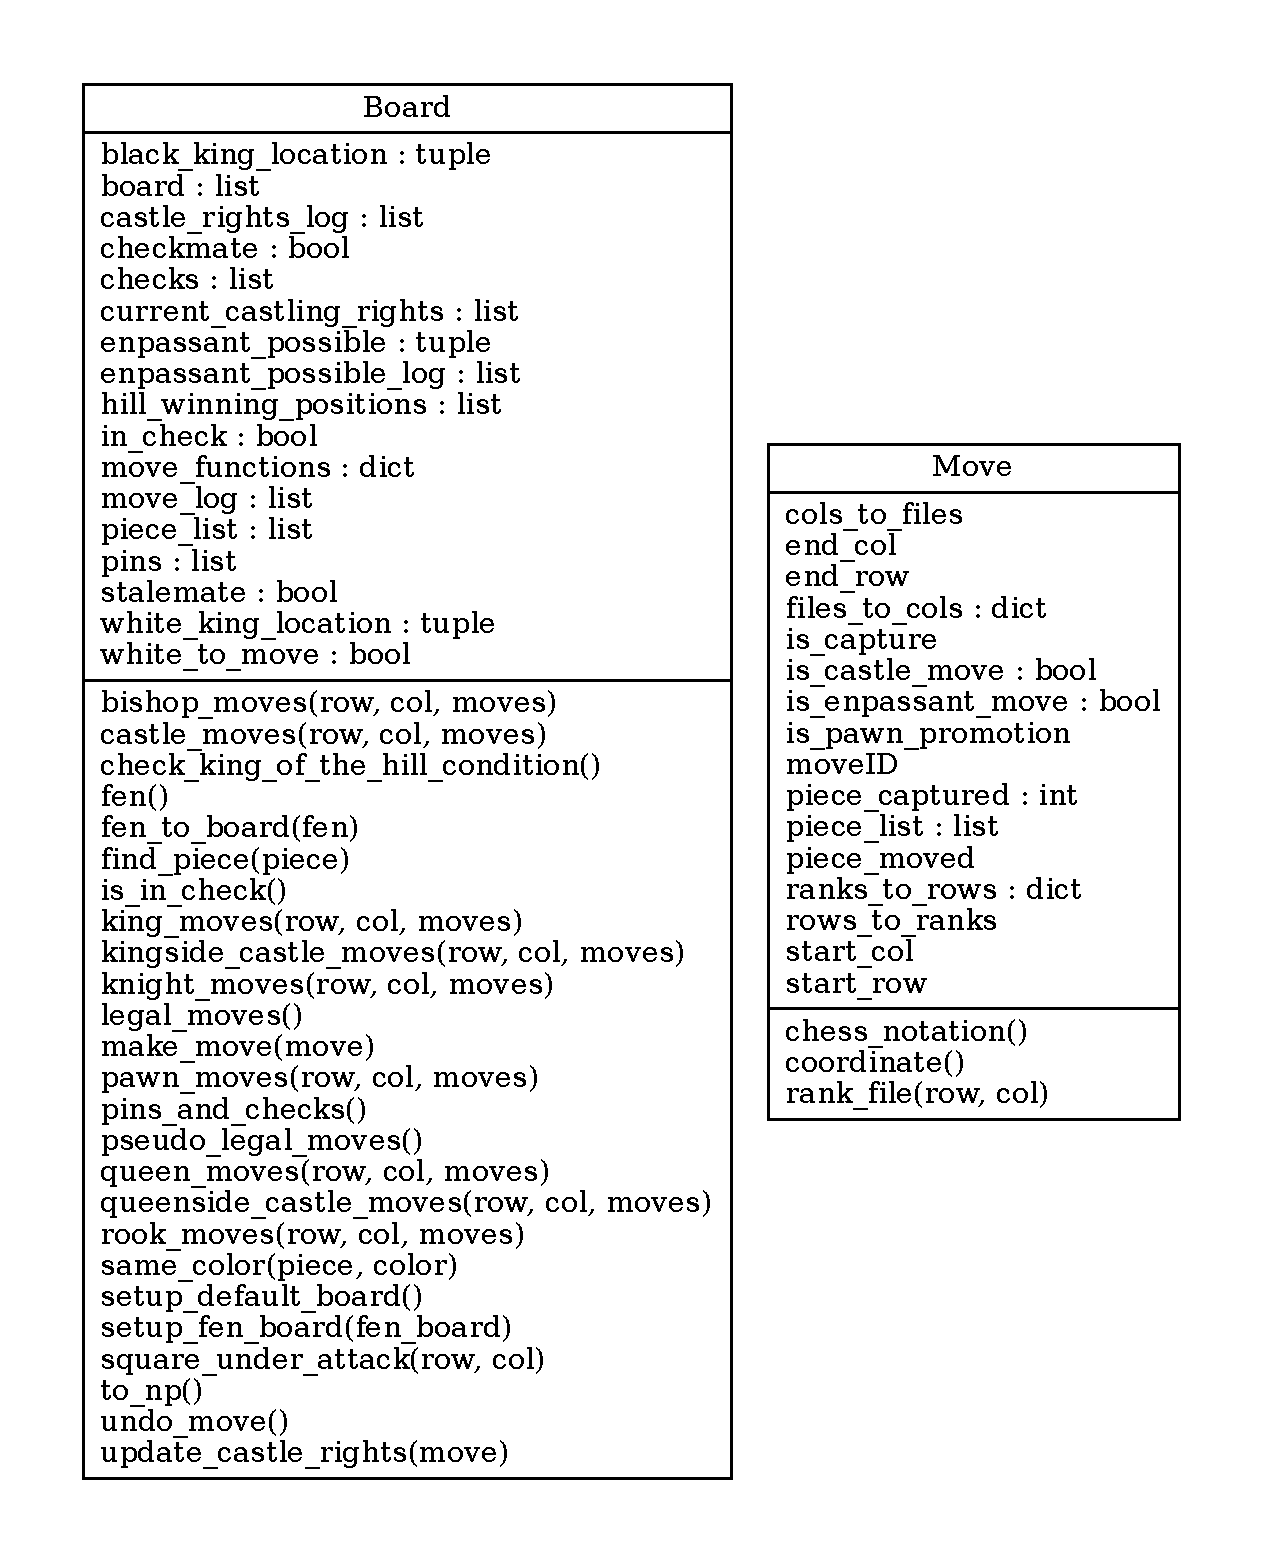
\includegraphics[width=0.7\linewidth, page=1]{reference/pics/class-diagram.pdf}
	\caption{Class diagram of the chess backend in its latest state}
  \label{fig:class-diagram}
\end{figure}

	
\end{document}
